% This section allows you to use package options without loading all the packages individually
\PassOptionsToPackage{dvipsnames}{xcolor}
\PassOptionsToPackage{colorinlistoftodos, prependcaption}{todonotes}
\PassOptionsToPackage{export}{adjustbox}
\PassOptionsToPackage{natbibapa}{apacite}
\PassOptionsToPackage{english}{babel}
\PassOptionsToPackage{para}{footmisc}
\PassOptionsToPackage{acronym}{glossaries}
\PassOptionsToPackage{printonlyused}{acronym}
\PassOptionsToPackage{T1}{fontenc}
\PassOptionsToPackage{linktocpage = true}{hyperref}
\PassOptionsToPackage{utf8}{inputenc}
\PassOptionsToPackage{toctitles}{titlesec}

\documentclass[12pt, a4paper, twoside, openright, final]{report}

% Load all the packages required by the various bits of this template, and some useful stuff as well. If you need any other packages just add them to this list.
\usepackage{graphicx, makeidx, changes, amsmath, tocbibind, sectsty, fancyhdr, appendix, lipsum, afterpage, ifthen, xkeyval, xcolor, tikz, calc, listings, acronym, adjustbox, array, authblk, babel, stackengine, etoolbox, booktabs, regexpatch, caption, colortbl, dcolumn, footmisc, glossaries, calc, inputenc, longtable, lscape, multirow, parskip, overpic, siunitx, subfig, framed, pgfplots, xspace, xargs, sansmathfonts, fontenc, url, titlesec, enumitem, csquotes}
% Some packages insist on being loaded seperately
\usepackage[backend=biber, natbib, style=apa]{biblatex}
\usepackage{hyperref} % MUST load hyperref here, it's really fussy
\usepackage{technical/imasphdthesis} % This custom package sets up all the extraneous thesis stuff

% Export a biblatex file and add here, plus any manual references if needed
\addbibresource{other_content/thesis_refs_biblatex.bib} 
\addbibresource{other_content/manual-refs.bib}
\DefineBibliographyStrings{english}{%
    bibliography = {Global Reference List} % Set bibliography name
}

% If you want to generate an index you should include the following command and un-comment the \printindex command at the very end of this file. 
% An index is an alphabetical list of words/expressions with the page numbers where they can be found. Use \index{} in the main text to add a word to the index.
\makeindex

%%%%%%%%%%%%%%%%%%%%%%%%%%%%%%%%%%%%%%%%%%%%%%%%%%
% Uncommenting this next line will make all your custom todo-notes maaaaaaaagically disappear!
%\renewcommand{\todo}[1]{\vphantom{\hphantom{#1}}}
%%%%%%%%%%%%%%%%%%%%%%%%%%%%%%%%%%%%%%%%%%%%%%%%%%

\begin{document}

\title{MY THESIS IS GOING TO BE AWESOME} % Use all capital letters
\author{Ms Bea A. Mazing} % Use mixed upper & lower case
\prevdegrees{M.Sc. B.Sc. Hons} % Specify previous degrees, use mixed upper & lower case
\advisor{Professor H. Hound} % example: Professor Lawrence K. Forbes
\dept{Fisheries \& Aquaculture}
\date{} % alternatively, manually include month & year of your thesis submission as below
%\submitdate{January, 2025} 

% Set headers for preface sections (these are not required to be all caps any more)
\settocname{Table of Contents} % Set the table of contents name
\setlofname{List of Figures} % Set the list of figures name
\setlotname{List of Tables} % Set the list if tables name
\setindexname{Index} % Set the index name

% Custom commands are seperated out for neatness. Put any custom commands you want to include in here
% For custom commands

\newcommand{\bfx}{{\ensuremath{\mathbf{x}}}}
\newcommand{\bfy}{{\ensuremath{\mathbf{y}}}}

% These columns replace the original c, l and r column types with C{xcm}, R{xcm} and R{xcm} columns that will wrap text
\newcolumntype{R}[1]{>{\raggedleft\arraybackslash}p{#1}}
\newcolumntype{L}[1]{>{\raggedright\arraybackslash}p{#1}}
\newcolumntype{C}[1]{>{\centering\arraybackslash}p{#1}}
\newcolumntype{X}[1]{>{\centering \arraybackslash}m{#1}}

% The original \paragraph command doesn't act as a miniheading - this does
\titlespacing*{\paragraph}{0pt}{3.25ex plus 1ex minus .2ex}{1em}
\newcommand{\myparagraph}[1]{\paragraph{#1}\mbox{}\\}

% I like to put little icons inline, especially in figure legends. This allows that with \icon{image_file.png}
\newcommand*{\icon}[1]{%
    \raisebox{-0.2\baselineskip}{%
        \includegraphics[height=0.75\baselineskip,
                         width=0.75\baselineskip,
                         keepaspectratio]{#1}}}

\newcommand{\note}[1]{\todo{#1}}
\newcommand{\fix}[1]{\todo{#1}}

% Super useful!! Species commands that allow you to use a one-word command for each species. The first time its used in the document it will give the full name and attribution, then all other times it will give the abbreviated name in italics.
\newcommand{\species}[4]{%
  \newcommand{#1}{\gdef#1{\textit{#4}\xspace}\textit{#2}\xspace#3\xspace}}
% Usage:
% \species{\<customcommand>}{<full~binomial~name>}{<species~citation>}{<abbreviated~binomial~name>}

% Here are the ones I've used....
\species{\macrocystis}{Macrocystis~pyrifera}{(L.)~C.~Agardh}{M.~pyrifera}
\species{\ecklonia}{Ecklonia~radiata}{(C.~Agardh)~J.~Agardh}{E.~radiata}
\species{\lessonia}{Lessonia~corrugata}{A.H.S.~Lucas}{L.~corrugata}
\species{\asalmon}{Salmo~salar}{L.}{S.~salar}
\species{\saccharina}{Saccharina~latissima}{(L.)~C.~E.~Lane,~C.~Mayes,~Druehl~\&~G.~W.~Saunders}{S.~latissima}
\species{\mytilus}{Mytilus~edulis}{L.}{M.~edulis}

% These are the citation alias commands - see citation_aliases.tex for details
\newcommand{\mycitet}[1]{%
    \citetalias{#1}~(\citeyear{#1})}
\newcommand{\mycitep}[1]{%
    (\citetalias{#1},~\citeyear{#1})}
\newcommand{\mycitealt}[1]{%
    \citetalias{#1}~\citeyear{#1}}
    
% end of new commands

% Aliases allow you to define acronyms or shortened author names for use in in-text citations while keeping the full name in the reference list (e.g. CSIRO, IMAS, FAO). See the file for details.
% Use these with \mycitet, \mycitep, and \mycitealt
% e.g. \mycitep{petuna_aquaculture_pty_ltd_environmental_2017}

\defcitealias{australian_bureau_of_agricultural_and_resource_economics_and_sciences_australian_2020}{ABARES} % Australian fisheries and aquaculture outlook 2020
\defcitealias{australian_bureau_of_agricultural_and_resource_economics_and_sciences_australian_2021}{ABARES} % Australian fisheries and aquaculture statistics 2021
\defcitealias{australian_bureau_of_agricultural_and_resource_economics_and_sciences_fishery_2019}{ABARES} % Fishery status reports 2019
\defcitealias{wageningen_university__research_processing_2022}{WUR}
\defcitealias{food_and_agriculture_organization_chapter_2003}{FAO}
\defcitealias{institute_for_marine_and_antarctic_studies_octopus_2020}{IMAS}
\defcitealias{integrated_marine_observing_system_zooplankton_2023}{IMOS}
\defcitealias{department_of_natural_resources_and_environment_salmon_2023}{DNRE}
\defcitealias{australian_bureau_of_statistics_station_2023}{BOM} % Station No. 094020
\defcitealias{petuna_aquaculture_pty_ltd_environmental_2017}{Petuna}
\defcitealias{tassal_group_ltd_environmental_2002}{Tassal}
\defcitealias{tassal_group_ltd_our_2022}{Tassal}
\defcitealias{tassal_group_ltd_our_2023}{Tassal}
\defcitealias{tassal_group_ltd_1h22_2022}{Tassal}
\defcitealias{tassal_group_ltd_annual_2010}{Tassal}
\defcitealias{tassal_group_ltd_annual_2021}{Tassal}
\defcitealias{tassal_group_ltd_bird_2023}{Tassal}
\defcitealias{tassal_group_ltd_seal_2023}{Tassal}



% Populates all text in the preface sections
\include{other_content/preface_text}

% \insertplain and \insertempty are two commands you might find useful. \insertplain inserts a single page that has no content but retains some of the formatting of the previous page (ie page numbers). \insertempty inserts a completely empty page with nothing on it at all.

% Start of preface sections - comment out any optional sections you don't need or don't want to load right now for speed
\singlespace
\titlepg % Title page (required) including empty page after
\dedication % Dedication of thesis (optional). Not currently in template, but this is where it would go.
\signaturepage % Declaration of originality and copyright (required)
%\publishedstatement % Statement regarding published work (optional). Not currently in template, because I didn't use one, but this is where it would go. 
\coauthorship % Optional, only if you need to declare co-authorship
%\ethicalconduct % Statement regarding ethical conduct. Not currently in template, because I didn't use one, but this is where it would go.
\acknowledgements % Acknowledgments page (optional)
\thesisquote % Optional
\generalabstract % Abstract to be bound with thesis (required)
\insertplain

% Contents, lists of tables and figures (required)
\pagestyle{fancy}
\fancyhf{}
\fancyhead[L]{} \fancyhead[C]{} \fancyhead[R]{\nouppercase{\rightmark}}
\fancyfoot[RO, LE]{\thepage}
\renewcommand{\headrulewidth}{0.4pt}

\makeatletter
\renewcommand{\@makechapterhead}[1]{%
	{\parindent \z@ \raggedright \reset@font
		\normalfont \Huge \bfseries \rmfamily  #1\par
		\nobreak
		\rule{\linewidth}{0.4pt}
		\vskip 15\p@
}}
\renewcommand{\@makeschapterhead}[1]{%
	{\parindent \z@ \raggedright \reset@font
		\normalfont \Huge \bfseries \rmfamily  #1\par
		\nobreak
		\rule{\linewidth}{0.4pt}
		\vskip 15\p@
}}
\makeatother

\tableofcontents 
\listoffigures 
\listoftables 
% The list of acronyms isn't a "proper" chapter so it doesn't automatically open on an odd page like the others and might need these bookends. Remove them if necessary.
    \clearpage \null \newpage 
\listofacronyms
    \clearpage \null \newpage

%% Main chapter texts (required, obviously)
% I've customised my lists of tables and figures to include the chapters as sub-headings so you know where the figures/tables sit. 
% However, if a chapter has no figures/tables, that looks weird. As a workaround, the formatting file below can be copied, modified and re-inserted before any chapter to change which headers appear in which lists. 
% Just some general formatting for the main chapters. 
\pagestyle{fancy}
\pagenumbering{arabic}

% My general introduction has figures but no tables
\makeatletter
\renewcommand{\@makechapterhead}[1]{%
    % Comment out next line to remove the chapter from the list of figures
    \addcontentsline{lof}{chapter}{\protect\numberline{\thechapter}#1}
    % Comment out next line to remove the chapter from the list of tables
    %\addcontentsline{lot}{chapter}{\protect\numberline{\thechapter}#1}
	{\parindent \z@ \raggedright \reset@font
		\ifnum \c@secnumdepth >\m@ne
			\normalfont \bfseries \LARGE \rmfamily \scshape \@chapapp{} \thechapter
			\par
			\vskip 15\p@
		\fi
		\normalfont \Huge \bfseries \rmfamily  #1\par
		\nobreak
		\rule{\linewidth}{0.4pt}
		\vskip 15\p@
}}

\renewcommand{\@makeschapterhead}[1]{%
    % Comment out next line to remove the chapter from the list of figures
    \addcontentsline{lof}{chapter}{\protect\numberline{\thechapter}#1}
    % Comment out next line to remove the chapter from the list of tables
    %\addcontentsline{lot}{chapter}{\protect\numberline{\thechapter}#1}
	{\parindent \z@ \raggedright \reset@font
		\ifnum \c@secnumdepth >\m@ne
			\normalfont \bfseries \LARGE \rmfamily \scshape \@chapapp{} \thechapter
			\par
			\vskip 15\p@
		\fi
		\normalfont \Huge \bfseries \rmfamily  #1\par
		\nobreak
		\rule{\linewidth}{0.4pt}
		\vskip 15\p@
}}
\makeatother
 

% I've included the chapter titles in this document INSTEAD of in the seperate tex files. That way, you can comment out the main content here for faster/piecemeal compiling but keep all the headings and lables, and the chapter numbers don't get messed up. 
\chapter{General introduction and structure of this thesis
        }\label{chap:gen-intro}
\section{First section}
Let's get writing. 
\note{This is a note - it's pretty cool and it stands out.}

\section{Second section - this one has equations}
Writing equations is really easy, and you can refer back to them from any chapter (Equation \ref{1-equ:relativity}).
%
\begin{equation}
    \label{1-equ:relativity}
    E = mc^2
\end{equation}
%
You can also refer to figures. You can try to force figures to go in the text exactly where you place them, but most of the time it's better to place them right after you first mention it, make a \textit{suggestion} of its placement (here, top of page, bottom of page, or whole page) and let \LaTeX place it at the next available spot that doesn't interrupt flow too much. (see Figure \ref{1-fig:boats}). 
%
\begin{figure}[htbp]
    \centering
    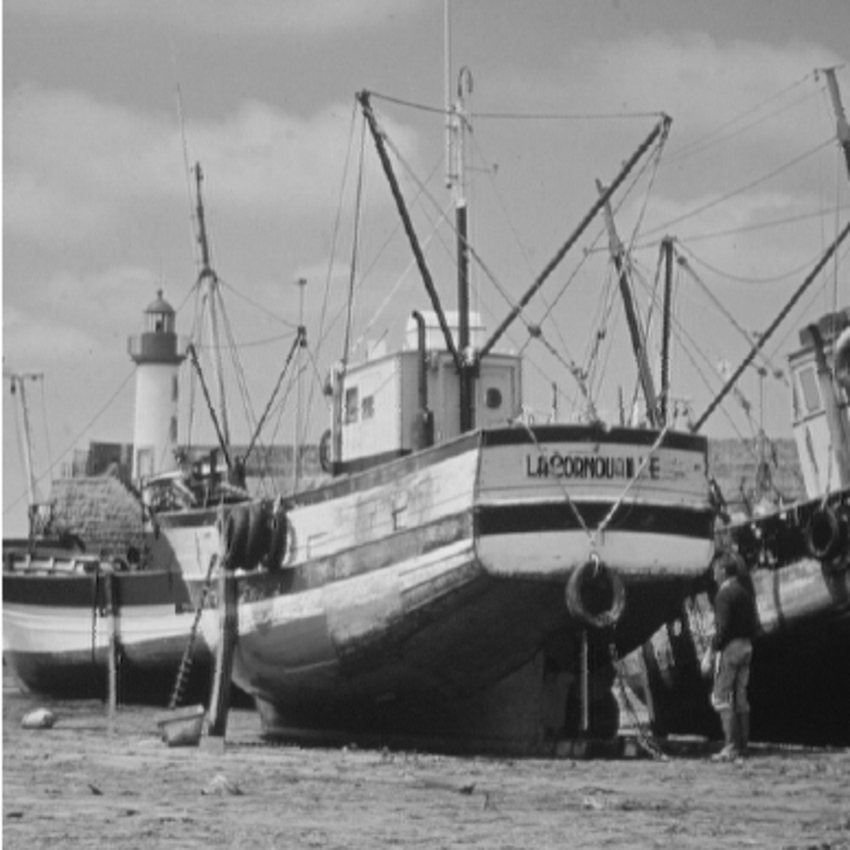
\includegraphics[width=0.75\linewidth]{figures/C1_general_intro/boat.png}
    \caption[This is a figure with an alternative caption]{This is a figure, with a long and descriptive caption. Figure captions should be able to stand on their own so they can get long. Maybe this was adapted from \citet{alexander_navigating_2016}, or maybe it relates to Equation \ref{1-equ:relativity} - who knows? All I know is that I don't want all this to appear in this Table of Figures.} 
    \label{1-fig:boats}
\end{figure}
%
You can even flow your text around a figure while writing and \LaTeX will stick the text blocks together like normal. 

\subsection{A subsection --- with acronyms!}
I may need to define some acronyms in the acronym document, like \ac{hab} and \ac{do}. Then I can talk about the effect of \ac{do} on \acp{hab} later on and everyone will know what I'm talking about. Did you notice that \ac{hab} was pluralised back there? What if I want a customised plural, like for \ac{ena}? I can do that --- the full version becomes \ac{ena} and the short version stays as \ac{ena}. I can also force capitalisation with \Ac{do}. 

\subsection{Here's another subsection --- with lists!}
\begin{enumerate}
    \item This is a list of things. I like to put lots of lists in my writing and I really with scientific writing would catch up with my genius.
    \item A list of aims maybe?
    \begin{enumerate}
        \item Nested lists automatically choose appropriate letters
        \item And always look nice
        \begin{itemize}
            \item And you can nest itemised lists and well.
            \item That's...
        \end{itemize}
        \item Super...
    \end{enumerate}
    \item Neat!
\end{enumerate}

\section{Primary aims and structure of this thesis}
\note{This is how my thesis is structured.}
The primary aims of this thesis were to....

\textbf{Chapter \ref{chap:1st-data}} aimed to...

\textbf{Chapter \ref{chap:2nd-data}} aimed to...

\textbf{Chapter \ref{chap:3rd-data}} aimed to...

Finally, \textbf{Chapter \ref{chap:gen-disc}} aimed to...


\chapter{This is the full title of my first data chapter
        }\label{chap:1st-data}
% If you've already published a chapter of your thesis before submission then inserting it unchanged can make the flow seem disruptive. Previous IMAS students (e.g. Keeley, 2015) have included a little ``framed abstract'' before published chapters to briefly contextualise the chapter in terms of the rest of the thesis.
% If you want to do that, then add these next lines before the chapter begins:
\begin{framed}
\lipsum[3] % Replace with actual content, obviously
\end{framed}\newpage
\section{Introduction}
You know how it works now....

\section{Methods}

Figure \ref{2-fig:sites} is a map and it's great.

\begin{figure}[htbp]
    \centering
    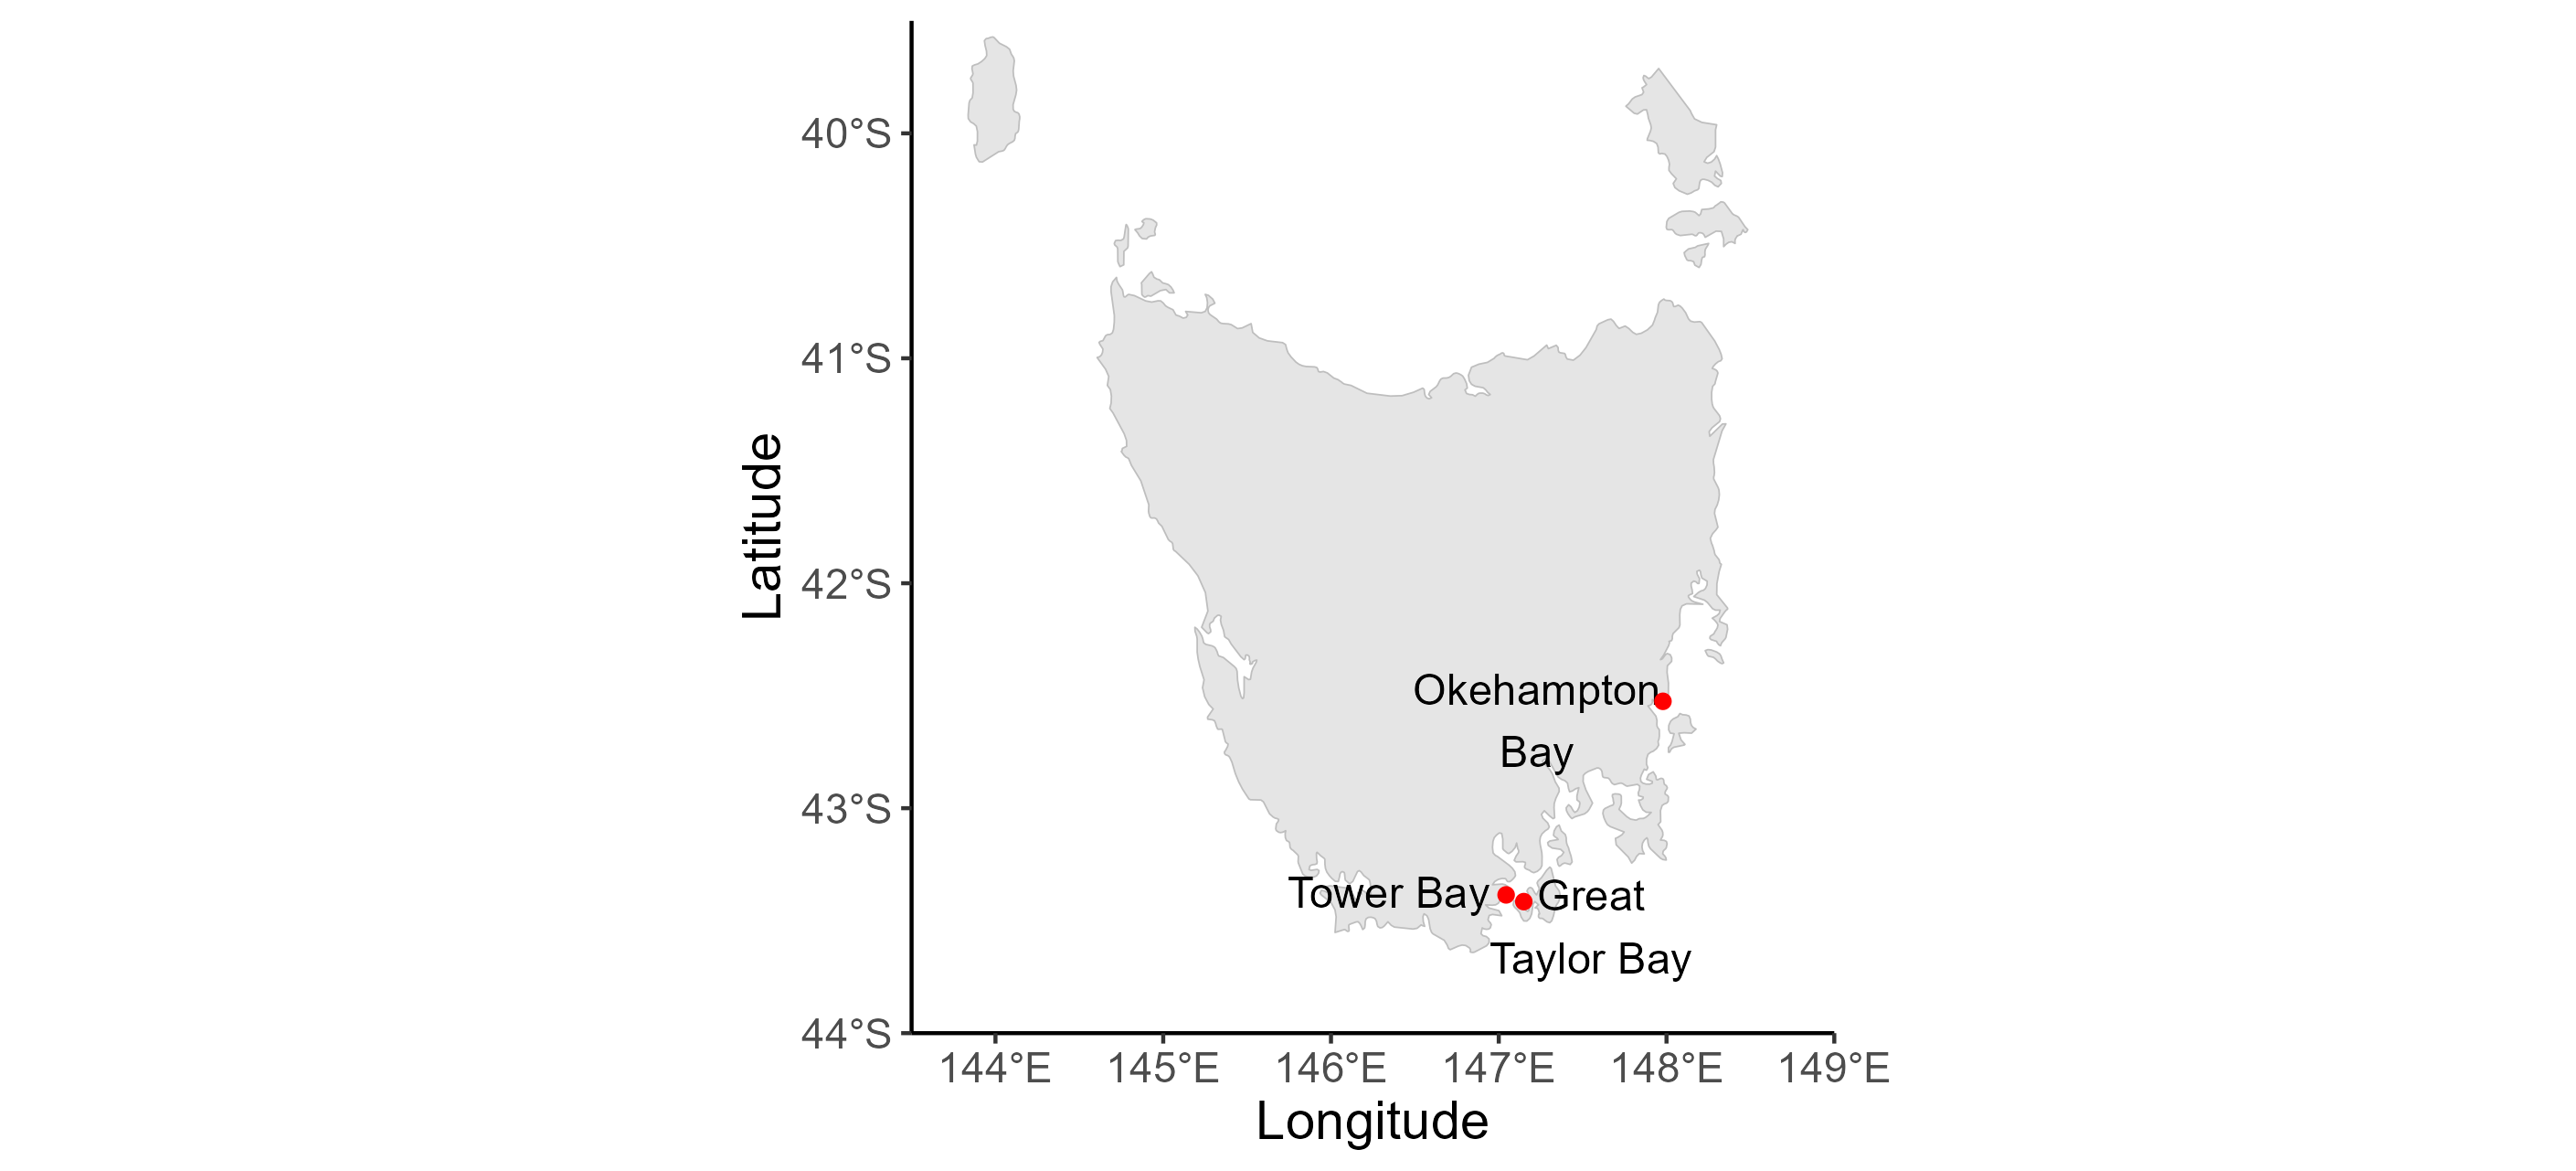
\includegraphics[width=0.85\linewidth, trim={4cm 0cm 4cm 0cm}, % trim={left bottom right top}
        clip]{figures/C2_1st_data_chapter/map.png}
    \caption[
        The three field sites from which my data was collected
    ]{
        The three field sites from which my data was collected. Adapted from \citet{biancacci_optimisation_2022}.
    } \label{2-fig:sites}
\end{figure}

\subsubsection{Experimental setup}
This new paragraph shows how to set \index{index items}index items
and \index{index items!subindex items} subindex items.

\subsection{Data collection and analysis}
I used the ``input'' command to put a big table in here because otherwise it takes up a lot of room in my code.
You can also try putting this table in landscape mode, but your text can't flow around it like a figure. 

%\begin{landscape}
    {\centering \small
\begin{longtable}{c l p{0.42\linewidth} r r r}
    \caption[
        A very fancy table
    ]{
        Summary of things! This table will span across multiple pages automatically, so that's nice. It will also place the top and bottom lines automatically at the page breaks.
    } \label{2-tab:summary} \\
    %
    \toprule
    Method & Unit & Description & Group 1 & Group 2 & Group 3 \\
    \midrule
    \endfirsthead
    %
    \caption[]{Notice that this caption is different than the first one. I like to replace the (usually long) first caption with a simple ``Table \thetable\ cont.''} \\
    %
    \toprule
    Symbol & Unit & Description & Group 1 & Group 2 & Group 3 \\
    \midrule
    \endhead
    %
    \bottomrule \endfoot
    \bottomrule \endlastfoot
    %
    % Start of main table
     & unit & This description is long. This column stays the same width, but the others will adjust to their contents. 
        & 100\footnote{\citet{smart_seasonal_2022}\label{smart2010}} 
        & 200\footref{smart2010}
        & 300\footref{smart2010} \\
    $B_a$ & unit & This description is long. This column stays the same width, but the others will adjust to their contents. 
        & 100\footnote{\citet{kopczak_variability_1994}\label{kopczak1994}} 
        & 200\footref{kopczak1994}
        & 300\footnote{\citet{miller_ecophysiology_2003}\label{miller2003}} \\
    $C_a$ & unit & This description is long. This column stays the same width, but the others will adjust to their contents.  
        & 100\footref{miller2003}
        & 200\footnote{\citet{wickham_species-specific_2019}\label{wickham2019}}
        & 300\footref{kopczak1994} \\
    $D_a$ & unit & This description is long. This column stays the same width, but the others will adjust to their contents.  
        & 100\footnote{\citet{zuniga_seasonal_2020}\label{zuniga2020}}
        & 200\footref{wickham2019}
        & 300\footref{zuniga2020} \\
    $E_a$ & unit & This description is long. This column stays the same width, but the others will adjust to their contents.  
        & 100\footref{zuniga2020} 
        & 200\footref{miller2003}
        & 300\footref{zuniga2020} \\
    $F_a$ & unit & This description is long. This column stays the same width, but the others will adjust to their contents.  
        & 100\footref{miller2003}
        & 200\footnote{\citet{trancoso_modelling_2005}\label{trancoso2005}}
        & 300\footref{trancoso2005} \\
    $G_a$ & unit & This description is long. This column stays the same width, but the others will adjust to their contents. 
        & 100\footnote{\citet{wheeler_effect_1980}\label{wheeler1980}}
        & 200\footref{trancoso2005} 
        & 300\footnote{\citet{biancacci_optimisation_2022}\label{biancacci2022}} \\
    $H_a$ & unit & This description is long. This column stays the same width, but the others will adjust to their contents.  
        & 100\footnote{\citet{enriquez_light_1994}\label{enriquez1994}}
        & 200\footref{biancacci2022} 
        & 300\footref{zuniga2020} \\
    $I_a$ & unit & This description is long. This column stays the same width, but the others will adjust to their contents.   
        & 100\footnote{\citet{gao_growth_2016}\label{gao2016}}
        & 200\footnote{\citet{buschmann_opportunities_2008}}
        & 300\footref{gao2016} \\ 
    $J_a$ & unit & This description is long. This column stays the same width, but the others will adjust to their contents.  
        & 100\footref{wickham2019}
        & 200\footnote{\citet{zimmerman_episodic_1984, zimmerman_situ_1986}}
        & 300\footnote{\citet{bearham_temperature_2013}} \\
    $K_a$ & unit & This description is long. This column stays the same width, but the others will adjust to their contents. 
        & 100\footnote{See section \ref{chap:3rd-data}\label{igiveup}}
        & 200\footnote{\citet{fernandez_nitrogen_2020}\label{fernandez2020}}
        & 300\footnote{\citet{tala_growth_2005}\label{tala2005}} \\* % I've decided I don't want the page break to happen here.
    $L_a$ & unit & This description is long. This column stays the same width, but the others will adjust to their contents.  
        & 100\footref{biancacci2022} 
        & 200\footnote{\citet{bolton_temperature_1987}\label{bolton1987}}
        & 300\footref{trancoso2005} \\
    $M_a$ & unit & This description is long. This column stays the same width, but the others will adjust to their contents.  
        & 100\footref{gao2016}  
        & 200\footref{smart2010}
        & 300\footnote{\citet{james_thermal_2023}\label{james2023}} \\
    $N_a$ & unit & This description is long. This column stays the same width, but the others will adjust to their contents.  
        & 100\footref{james2023}  
        & 200\footref{bolton1987}  
        & 300\footnote{\citet{hernandez-carmona_effect_2001}\label{hernandez2001}} \\
    $O_a$ & unit & This description is long. This column stays the same width, but the others will adjust to their contents.  
        & 100\footref{miller2003}
        & 200\footnote{\citet{staehr_physiological_2009}}
        & 300\footnote{\citet{mabin_physiological_2019}\label{mabin2019}} \\
    $P_a$ & unit & This description is long. This column stays the same width, but the others will adjust to their contents.  
        & 100\footref{mabin2019}  
        & 200\footref{hernandez2001}  
        & 300\footref{smart2010} \\
    $Q_a$ & unit & This description is long. This column stays the same width, but the others will adjust to their contents.  
        & 100\footref{biancacci2022} 
        & 200\footref{wickham2019}
        & 300\footref{bolton1987} \\
    $R_a$ & unit & This description is long. This column stays the same width, but the others will adjust to their contents.  
        & 100\footref{smart2010}
        & 200\footref{smart2010}
        & 300\footref{gao2016} \\
    $S_a$ & unit & This description is long. This column stays the same width, but the others will adjust to their contents.  
        & 100\footref{mabin2019}  
        & 200\footref{james2023}  
        & 300\footref{zuniga2020} \\
    $T_a$ & unit & This description is long. This column stays the same width, but the others will adjust to their contents.  
        & 100\footref{zuniga2020} 
        & 200\footref{trancoso2005} 
        & 300\footref{hernandez2001} \\
    $U_a$ & unit & This description is long. This column stays the same width, but the others will adjust to their contents.  
        & 100\footref{hernandez2001}  
        & 200\footref{tala2005}  
        & 300\footref{wickham2019} \\
\end{longtable}
}
%\end{landscape}

\section{Results}

\subsection{Subset 1}

Sometimes subfigures are needed, and you can do it with Figures \ref{2-fig:parrots}A \& B.
However, you might just output the figures from R with the As and Bs already on them and put them in here as-is. 

\begin{figure}[hbtp]
    \centering
    \begin{overpic}[width=0.48\linewidth, trim={1.5cm 0cm 1cm 0cm}, clip%,grid, tics = 10
        ]{figures/C2_1st_data_chapter/parrots.jpg}
        \put(-5,65) {\normalsize\textbf{A}}
    \end{overpic}
    \begin{overpic}[width=0.48\linewidth, trim={1.5cm 0cm 1cm 0cm}, clip%,grid, tics = 10
        ]{figures/C2_1st_data_chapter/parrots.jpg}
        \put(-5,65) {\normalsize\textbf{B}}
    \end{overpic}
    \begin{overpic}[width=0.97\linewidth, trim={0cm 0cm 0cm -0.1cm}, clip%, grid, tics = 5
        ]{figures/C2_1st_data_chapter/parrots.jpg}
        \put(-2.5,57.5) {\normalsize\textbf{C}}
    \end{overpic}
    \caption[
        Example of sub-figures
    ]{
        Sub-figures can be put side-by-side, and you can use trimming and grids to get the sizing and scaling right.
    }\label{2-fig:parrots}
\end{figure}

\subsection{Subset 2}

\begin{landscape}
\begin{figure}[p]
    \centering
    %
    \begin{overpic}[width=0.4\linewidth%, grid, tics = 10 
                    , trim={-2.5cm 2.5cm 0cm -0.5cm} % left bottom right top
                    , clip
        ]{figures/C2_1st_data_chapter/liopleurodon.jpg}
        \put (-6, 55) {\normalsize\textbf{A}}
    \end{overpic}
    %
    \begin{overpic}[width=0.4\linewidth%, grid, tics = 10
                    , trim={-2.5cm 2.5cm 0cm -0.5cm} % left bottom right top
                    , clip
        ]{figures/C2_1st_data_chapter/liopleurodon.jpg}
        \put (-6, 55) {\normalsize\textbf{B}}
    \end{overpic}
    %
    \begin{overpic}[width=0.4\linewidth%, grid, tics = 10
                    , trim={-2.5cm 2.5cm 0cm -0.5cm} % left bottom right top
                    , clip
        ]{figures/C2_1st_data_chapter/liopleurodon.jpg}
        \put (-6, 55) {\normalsize\textbf{C}}
    \end{overpic}
    %
    \begin{overpic}[width=0.4\linewidth%, grid, tics = 10
                    , trim={-2.5cm 2.5cm 0cm -0.5cm} % left bottom right top
                    , clip
        ]{figures/C2_1st_data_chapter/liopleurodon.jpg}
        \put (-6, 55) {\normalsize\textbf{D}}
    \end{overpic}
    %
    \caption[IT'S A LIOPLEURODON CHARLIE]{Landscape, baby! You can trim and clip figures in Latex if you want to, although honestly it's a lot easier to do the subfigure layouts in ggplot2 and then just bring the whole picture into Latex.}
    \label{2-fig:liopleurodon}
    %
\end{figure}
\end{landscape}

\clearpage
\section{Discussion}
\subsection{I have so much to talk about}
\lipsum[1][]

\subsection{You can't shut me up}
\lipsum[3][]

\subsubsection{Just one more thing}
\lipsum[5][]


\chapter{This is the title of my second data chapter
        }\label{chap:2nd-data}
\section{Introduction}
\lipsum[8]

\section{Methods}

\subsection{Data collection and analysis}

\subsubsection{Statistical analysis}

\section{Results}

\section{Discussion}
\lipsum[5][]

    
\chapter{This is the title of my third data chapter
        }\label{chap:3rd-data}
\begin{framed}
Mini-abstract.
\end{framed}

\newpage
\section{Introduction}
\lipsum[8]

\section{Methods}

\subsection{Data collection and analysis}

\subsubsection{Statistical analysis}

\section{Results}

\clearpage
\section{Discussion}
\lipsum[5][]

    
\chapter{General discussion and synthesis of findings
        }\label{chap:gen-disc}
\section{Aaaaand it's the end.}
Here's yet another \index{section}section with an appropriate
index entry.



% Reference list (required)
% Slight changes to the headers
\fancyhead[L]{} \fancyhead[C]{} \fancyhead[R]{\nouppercase{\rightmark}}

\makeatletter
\renewcommand{\@makechapterhead}[1]{%
	{\parindent \z@ \raggedright \reset@font
		\normalfont \Huge \bfseries \rmfamily  #1\par
		\nobreak
		\rule{\linewidth}{0.4pt}
		\vskip 15\p@
}}
\renewcommand{\@makeschapterhead}[1]{%
	{\parindent \z@ \raggedright \reset@font
		\normalfont \Huge \bfseries \rmfamily  #1\par
		\nobreak
		\rule{\linewidth}{0.4pt}
		\vskip 15\p@
}}
\makeatother

\printbibliography

% Index (optional)
\printindex

% Appendices (optional)
\appendix 
\fancyhead[L]{Chapter \thechapter} \fancyhead[C]{} \fancyhead[R]{\nouppercase{\rightmark}}

\makeatletter
\renewcommand{\@makechapterhead}[1]{%
    \addcontentsline{lof}{chapter}{\protect\numberline{\thechapter}#1}
    \addcontentsline{lot}{chapter}{\protect\numberline{\thechapter}#1}
	{\parindent \z@ \raggedright \reset@font
		\ifnum \c@secnumdepth >\m@ne
			\normalfont \bfseries \LARGE \rmfamily \scshape \@chapapp{} \thechapter
			\par
			\vskip 15\p@
		\fi
		\normalfont \Huge \bfseries \rmfamily  #1\par
		\nobreak
		\rule{\linewidth}{0.4pt}
		\vskip 15\p@
}}
\renewcommand{\@makeschapterhead}[1]{%
	{\parindent \z@ \raggedright \reset@font
		\ifnum \c@secnumdepth >\m@ne
			\normalfont \bfseries \LARGE \rmfamily \scshape \@chapapp{} \thechapter
			\par
			\vskip 15\p@
		\fi
		\normalfont \Huge \bfseries \rmfamily  #1\par
		\nobreak
		\rule{\linewidth}{0.4pt}
		\vskip 15\p@
}}

\pagestyle{fancy}
\fancyhead[L]{Appendix \thechapter \chaptermark{}} \fancyhead[C]{} \fancyhead[R]{}
%\fancyfoot[LE]{\thepage} \fancyfoot[C]{} \fancyfoot[RO]{\thepage}
\normalsize
\singlespace
\makeatother

\chapter{Chapter \ref{chap:1st-data} appendix
        }\label{app:A1_app_name}
\section{First section of the appendix}
\begin{equation}
    G_{\mu\nu}=\frac{8\pi G}{c^4}T_{\mu\nu}
\end{equation}






\chapter{Statistical results for Chapter \ref{chap:2nd-data}
        }\label{app:A2_app_name}
\section{Discrepancies between the approach taken here and reality}
I swear to God, this is a real section title in my thesis. Where else would I put it but an appendix?



\chapter{Additional and supporting information for \ref{chap:2nd-data}
        }\label{app:A3_app_name}
\section{Final appendix}
It's the end. Go home.






\end{document}